\documentclass[11pt,a4paper]{article}
\usepackage[margin=2.3cm]{geometry}
\usepackage{graphicx,booktabs,amsmath,xcolor,enumitem}
\usepackage[hidelinks]{hyperref}
\setlist{itemsep=2pt,topsep=3pt}
\setlength{\parskip}{4pt}\setlength{\parindent}{0pt}
\newcommand{\code}[1]{\texttt{#1}}
\title{Top-view kit: how to read the statistics}
\author{Renaud H\'edouin}
\date{27 November 2026}
\begin{document}\sloppy
\maketitle

This note explains the two statistical tables of the kit that are not self-explanatory,
\code{models\_coefficients.csv} and \code{models\_variance.csv}, and what the time effect means.
Numbers are from the segmentation model v7f, on the mixing index at 12\,mm
(\code{mix\_12mm}: 0 = colours in separate patches, 1 = colours placed at random).
The same reading applies to the other indices (\code{cellH\_26mm}, \code{strat\_rho}).

\section{Why a mixed model}

Our photos are not independent. Each nest is photographed several times (photo 1 to 4, sometimes 5--6),
each pair builds two nests (round 1, round 2), and pairs belong to three cohorts:
\[
\text{cohort} \;\supset\; \text{pair} \;\supset\; \text{nest (round 1, round 2)} \;\supset\; \text{photo (session 1, 2, 3, \dots)}
\]
Four photos of the same nest look alike. An ordinary regression would treat them as four
independent observations and give p-values that are far too small. A \emph{mixed model} handles
this by splitting the variation into two parts:
\begin{itemize}
\item \textbf{fixed effects}: what we want to test (cohort, round, time). Each gets a coefficient,
      a 95\,\% confidence interval and a p-value;
\item \textbf{random effects}: the grouping we are not testing but must respect. Each pair has its own baseline,
      and so does each nest within the pair. The model estimates how much these baselines vary.
\end{itemize}

\section{Reading the coefficients table}

Table~\ref{tab:coef} is \code{models\_coefficients.csv} for \code{mix\_12mm}, all 104 photos where mixing is defined.

\begin{table}[h]\centering\small
\begin{tabular}{lrcr}
\toprule
term & estimate & 95\,\% CI & p \\
\midrule
Intercept & 0.557 & [0.449; 0.665] & $<$0.001 \\
C(cohort)[T.2] & +0.001 & [$-$0.104; +0.105] & 0.99 \\
C(cohort)[T.3] & +0.066 & [$-$0.040; +0.172] & 0.22 \\
C(round)[T.2] & +0.081 & [$-$0.005; +0.167] & 0.064 \\
days & +0.0010 & [$-$0.0005; +0.0025] & 0.19 \\
\bottomrule
\end{tabular}
\caption{Mixed model \code{mix\_12mm \textasciitilde{} C(cohort) + C(round) + days}, all photos.}
\label{tab:coef}
\end{table}

\begin{itemize}
\item \textbf{Intercept}: the predicted value for the \emph{reference} situation, namely cohort 1, round 1,
      on the day of the nest's first top photo (day 0). Here 0.56: a first nest of cohort 1 starts moderately mixed.
\item \textbf{Every other row is a difference from that reference}, all else being equal.
      \code{C(cohort)[T.3]} $= +0.066$ means cohort 3 is on average 0.066 more mixed than cohort 1,
      at the same round and the same day. \code{T.2} reads ``level 2 compared to level 1''.
\item \textbf{days} is a slope: the change \emph{per day}. Over two weeks, multiply by 14.
\item \textbf{To predict} a situation, add up the rows that apply. Cohort 3, round 2, day 10:
      $0.557 + 0.066 + 0.081 + 10 \times 0.001 = 0.71$.
\item \textbf{The confidence interval} is the range of values compatible with the data.
      If it contains 0, the data cannot exclude ``no effect''.
      Round 2: $[-0.005; +0.167]$ just touches 0, so it is a trend, not a demonstrated effect.
\item \textbf{The p-value} is the probability of an effect at least this large if the true effect were zero.
      Below 0.05 is conventionally called significant. The CI says more: \emph{how big} the effect could be.
\end{itemize}

\textbf{The variance table} (\code{models\_variance.csv}) says where the remaining variation lies, once
the fixed effects are accounted for. For \code{mix\_12mm}: pair 0\,\%, nest 44\,\%, photo 56\,\%.
\begin{itemize}
\item \textbf{pair 0\,\%}: two nests of the same pair are not more alike than two nests of different pairs.
      There is no detectable ``pair style'' (consistent with the repeatability table).
\item \textbf{nest 44\,\%}: nests differ from each other, beyond cohort and round.
\item \textbf{photo 56\,\%}: a nest also changes between its own photos. This part includes real change over time,
      segmentation noise and changes of viewpoint.
\end{itemize}

\section{The time effect, and why photo 4 matters}

\begin{figure}[h]\centering
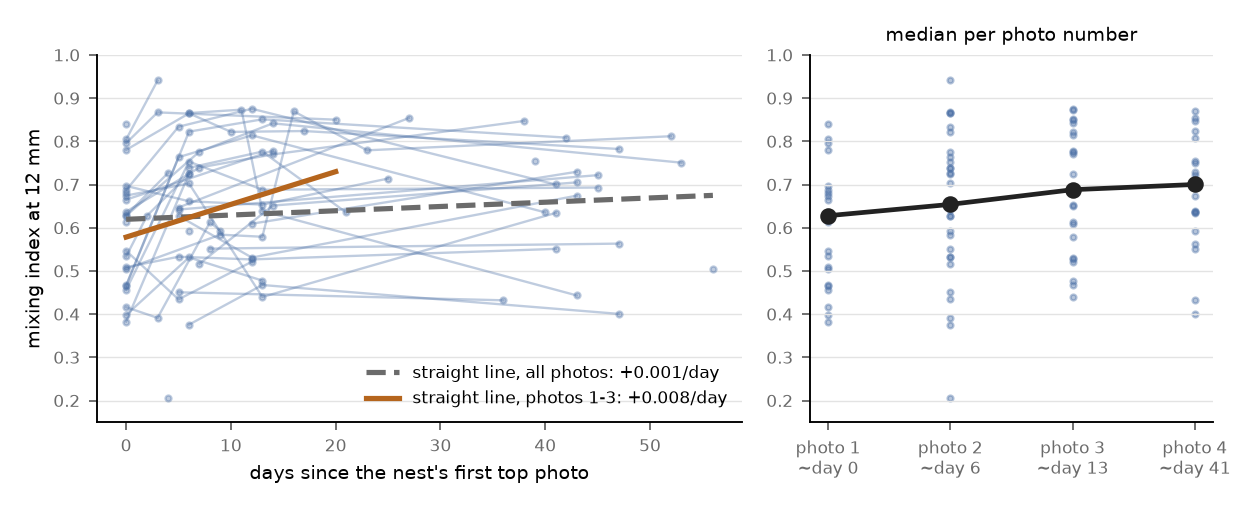
\includegraphics[width=\linewidth]{time_effect.png}
\caption{Left: mixing at 12\,mm of each photo against days since the nest's first top photo (one line per nest).
The two straight lines are the fitted time trends of the mixed model, with and without photos 4 and later.
Right: the same photos grouped by photo number (bar = median); photo 4 comes about four weeks after photo 3.}
\label{fig:time}
\end{figure}

With all photos, the \code{days} slope is small and uncertain: $+0.001$ per day, $p = 0.19$.
With photos 1--3 only (\code{--max-session 3}) it becomes $+0.0076$ per day, CI $[+0.003; +0.012]$, $p = 0.001$.
That is $+0.10$ over the two weeks between photo 1 and photo 3, a large change on a 0--1 scale.

The two results do not contradict each other. Figure~\ref{fig:time} shows why:
\begin{itemize}
\item mixing \textbf{rises during building}, between photo 1 (day 0) and photo 3 (about day 13);
\item then it \textbf{levels off}. Photo 4 is taken around day 41, after the eggs have hatched, and it is barely more mixed than photo 3;
\item a single straight line through day 0 to day 41 is pulled flat by these late photos. The model is then
      averaging a rise and a plateau, and finds a weak slope.
\end{itemize}

The option \code{--time session} confirms it without dropping any photo: it gives each photo number its own effect instead of a straight line.
On all photos, compared with photo 1, mixing is $+0.09$ at photo 2 ($p = 0.002$), $+0.11$ at photo 3 ($p < 0.001$)
and $+0.12$ at photo 4 ($p < 0.001$): the same rise and plateau. Photos 5--6 are too few to say anything.

\textbf{Why this is good news.}
\begin{itemize}
\item \textbf{The index measures something real.} Nests are built progressively, and the index follows the building:
      it increases while the birds work and stops when building stops.
      A metric dominated by noise would not show such an orderly pattern across nests.
\item \textbf{Biological reading.} The birds do not lay each new colour as a separate layer.
      They weave new string into what is already there, so colours get more intermixed as the nest grows.
      The plateau after laying fits building activity stopping.
\item \textbf{It shows that stage matters.} Comparing nests at different stages mixes up ``this nest is more mixed'' with
      ``this nest is further along''. Round and cohort comparisons should therefore keep a time term, and its form matters.
\end{itemize}

\textbf{Caveats.}
\begin{itemize}
\item \textbf{Visible colours change too.} The later colours are added on top, red after the first egg,
      and they change which colours are visible. The index is normalised by the colour proportions, but the photo-to-photo
      rise is partly a change in what we see from above. The side views will help to separate the two.
\item \textbf{Mixing is only defined with a second colour.} It is computed only when a second colour makes at least 10\,\% of the visible string,
      so very uniform photos (often photo 1, all orange) are left out.
\end{itemize}

\textbf{Practical advice}: to compare cohorts or rounds, use either \code{--max-session 3}
(building phase only, straight line in days is reasonable) or \code{--time session} (all photos, no straight-line assumption).
With the latter, the round-2 effect is $+0.07$, CI $[-0.02; +0.16]$, $p = 0.14$: still only a trend.

\section{Things to keep in mind}
\begin{itemize}
\item \textbf{The sample is small.} Mixing is defined on 104 photos of 37 nests and 24 pairs. Effects of a few hundredths are hard to detect,
      and an absence of significance is not an absence of effect. Look at the confidence intervals.
\item \textbf{Many tests.} With 10 scales, 3 indices and several subsets, some $p < 0.05$ will appear by chance.
      A pattern that holds across scales and subsets is more convincing than a single p-value.
\item \textbf{Strongly reduced subsets.} When a subset removes a variable (one round, one cohort), the corresponding row disappears.
      With a single round, each pair has one nest, so ``pair'' and ``nest'' variance can no longer be separated.
\end{itemize}

\end{document}
